% Paper 6 (T6) -- IEEE JBHI special issue "Integrating Imaging with Personalized Cardiovascular Medicine"
% Deadline 2026-10-15. Target: 8 pages (over-length charges start at page 9).
% Plan and word budgets: BENCHMARK-AND-PLAN-JBHI-2026-10-03.md
\documentclass[journal]{IEEEtran}
\usepackage{amsmath,amssymb}
\usepackage{graphicx}
\usepackage{booktabs}
\usepackage{siunitx}
\usepackage[hidelinks]{hyperref}

\begin{document}

\title{Boundary-Condition Tuning Conceals Topological Segmentation Error in Reduced-Order Coronary FFR}
% Working title; alternative from STUDY-PLAN-v2 sec. 0:
% "Matched at the Outlet, Wrong in the Tree: ..."

\author{Fadillah~Yamin,
        Mohd~Azan~Mohammed~Sapardi,
        Ming~Kwang~Tan,
        Xin~Wang,
        and~Mohd-Zulhilmi~Paiz~Ismadi%
\thanks{F. Yamin, X. Wang and M.-Z. P. Ismadi are with the Department of Mechanical Engineering, School of
Engineering, Monash University Malaysia, 47500 Bandar Sunway, Selangor, Malaysia (corresponding author:
M.-Z. P. Ismadi, e-mail: mohd.zulhilmi@monash.edu).}%
\thanks{M. A. Mohammed Sapardi is with the Department of Mechanical Engineering, Kulliyyah of Engineering,
International Islamic University Malaysia, 53100 Kuala Lumpur, Malaysia.}%
\thanks{M. K. Tan is with the Department of Mechanical Engineering, School of Engineering, Monash University
Malaysia, and the Department of Mechanical Engineering, Ming Chi University of Technology, New Taipei City 243,
Taiwan.}}

\markboth{IEEE Journal of Biomedical and Health Informatics}{Yamin \MakeLowercase{\textit{et al.}}: BC Tuning Conceals Segmentation Error in Coronary FFR}

\maketitle

\begin{abstract}
Fractional flow reserve computed from coronary computed tomography angiography depends on the segmented lumen and on
outlet boundary conditions that are derived from it and are often tuned to match perfusion. Whether tuning conceals
segmentation errors that change the treatment decision at 0.80 has not been tested. We
inserted stenoses into 150 coronary trees from a public dataset, applied four segmentation error types (a missed side
branch, a vessel break, a longer lesion and a narrowed taper), and recomputed fractional flow reserve with a
reduced-order model under three boundary-condition protocols: fixed, re-derived from the corrupted tree, and tuned to
the clean tree's territory perfusion. Two microvascular bed structures were analysed, and one case was also solved in three
dimensions. Topological errors changed the decision in 32--33\% of models with
fixed boundary conditions, against 6--10\% for calibre errors of inter-observer magnitude, which were close to the
variability of repeat invasive measurement. Re-deriving or tuning the boundary conditions reduced topological
decision changes to 5--20\%. Tuning, however, removed the perfusion mismatch that marked the error: 8--19\% of tuned
models with a topological error passed a perfusion check stricter than measurement repeatability while their
fractional flow reserve was wrong by more than 0.05. In the three-dimensional case, prescribed territory flows
reduced a missed-branch shift of 0.074 to below 0.001. A perfusion-matched coronary model can therefore pass
validation with a material error in the computed fractional flow reserve, and topological correctness of the
segmentation and the residual before tuning are needed to detect it.
\end{abstract}

\begin{IEEEkeywords}
Boundary conditions, coronary artery disease, fractional flow reserve, image segmentation, reduced-order modeling,
uncertainty.
\end{IEEEkeywords}

% ---------------------------------------------------------------------------------------------------------------
\section{Introduction}
\IEEEPARstart{F}{ractional} flow reserve (FFR) at or below 0.80 identifies a coronary stenosis for revascularisation
\cite{tonino2009}. Computed tomography (CT)-derived FFR estimates the same quantity without a pressure wire, by
solving a flow model on a lumen segmented from coronary CT angiography \cite{taylor2013,norgaard2014,itu2016}. The
model has two image-dependent inputs: the lumen geometry, which comes from segmentation, and the outlet boundary
conditions, which are derived from vessel calibre through allometric scaling and represent the microvascular bed
\cite{kim2010,murray1926}. An error in either input propagates to the computed FFR.

Published studies quantify the sensitivity of CT-derived FFR to lumen-radius uncertainty
\cite{sankaran2015tmi,sankaran2015cmame,fernandez2024} and compare the influence of geometry with that of boundary
conditions in coronary, pulmonary and cerebral vessels \cite{sankaran2016,tanade2022,colebank2019,korte2023}. These
studies perturb lumen calibre with the branching structure held fixed, and they report continuous sensitivity rather
than changes in the treatment decision. Automatic segmentation, however, also produces topological errors. In a
recent coronary benchmark, vessel breaks were present in the predictions of every evaluated method despite high
overlap scores \cite{bransby2026}. A missed side branch or a broken vessel removes part of the microvascular bed from
the model, which changes both the flow through the stenosis and the boundary conditions derived from the tree.

Model pipelines adjust boundary conditions so that predicted flow matches a physiological target, and this
adjustment can compensate for a geometric discrepancy. Re-tuning the microvascular resistance absorbed a change in
modelled side-branch flow with little change in diagnostic accuracy \cite{gosling2020}. Geometry and boundary
conditions have been adjusted jointly to match the same perfusion targets \cite{menon2024}. A change of the outlet
boundary-condition model left the area under the receiver operating characteristic curve unchanged (0.845) while
sensitivity changed from 58.1\% to 68.6\% \cite{fossan2026}. With outlet resistance held fixed, removal of a side
branch downstream of a stenosis changed FFR by 13--15\%, an effect that depends on whether resistance is re-tuned
\cite{gamage2022}. A model that matches its perfusion targets after re-tuning can therefore still carry a
segmentation error into the computed FFR. Whether this changes the decision at 0.80, and how often, has not been
tested under controlled conditions.

This study tests it. We inserted controlled stenoses into 150 real coronary trees from a public CT angiography
dataset, applied four segmentation error types, and recomputed FFR under three boundary-condition protocols: fixed,
re-derived from the corrupted tree, and re-tuned to the clean tree's territory perfusion (Fig.~\ref{fig:design}).
The cohort, design and
analysis plan were fixed before the ablation was run. The contributions are: (1) a controlled ablation of boundary-condition protocols against
topological and calibre segmentation errors, with the 0.80 decision as the outcome and a physiological-noise floor
as the comparator; (2) the proportion of models that pass a perfusion-based validation check while their FFR is
materially wrong; and (3) a three-dimensional computational fluid dynamics (CFD) case study of the same mechanism on
a segmented lumen.

% ---------------------------------------------------------------------------------------------------------------
\section{Methods}
\begin{figure*}[!t]\centering
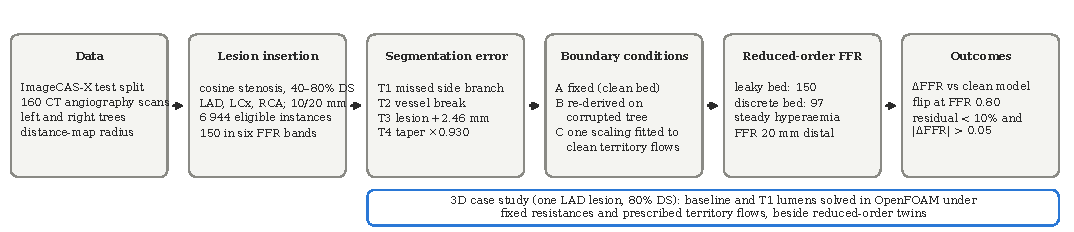
\includegraphics[width=\textwidth]{figures/fig1_design.pdf}
\caption{Study design. Each of 150 coronary instances is corrupted by four segmentation error types, solved under three
boundary-condition protocols in two bed structures, and compared with its own clean model. One instance is also
solved in three dimensions.}
\label{fig:design}
\end{figure*}
\subsection{Data and Cohort}
ImageCAS-X provides voxel-wise lumen and coronary-segment annotations, centerlines and surfaces for 800 CT angiography
scans of the ImageCAS dataset \cite{zeng2023,bransby2026,imagecasx_data}. We used its 160-scan test split, in which
each scan was re-annotated by a second analyst. Inter-observer agreement on this split was a Dice similarity
coefficient of 92.8\% and a 95th-percentile Hausdorff distance (HD95) of 2.46~mm \cite{bransby2026}. Each scan gives a
left and a right coronary tree. The local radius at each centerline point is the Euclidean distance transform of the
lumen mask, less half a voxel.

The natural cohort contains few lesions near the decision threshold, so stenoses were inserted into healthy vessels.
A host slot is a main vessel (left anterior descending, left circumflex or right coronary artery), a location
(20 or 45~mm from the vessel origin) and a length $L$ (10 or 20~mm). Eligible hosts had a healthy reference radius
$r_\mathrm{fit} \geq 1.0$~mm at the lesion centre, native narrowing below 40\% diameter stenosis (DS), a resolved
measurement point 20~mm distal to the lesion and a pre-insertion FFR of at least 0.90. The lesion is an axisymmetric
cosine narrowing,
\begin{equation}
\begin{aligned}
r'(s) &= \min\!\left(r,\; (1-w)\,r + w\,r_\mathrm{fit}\,(1-\mathrm{DS})\right),\\
w &= \tfrac{1}{2}\left[1+\cos\tfrac{2\pi (s-c)}{L}\right]
\end{aligned}
\end{equation}
for $|s-c|<L/2$, with severities of 40--80\% DS. The 6\,944 eligible instances were stratified into six bands of
baseline FFR (0.65--0.95), and 150 instances were selected (50 per vessel) from 108 trees of 93 patients. The
selected instances form a frozen, hashed list.

\subsection{Reduced-Order FFR Model}
The tree is a network with one node per centerline point. Each element has a Poiseuille resistance
$8\mu\,\Delta s/(\pi r^4)$ on the actual radius, and each stenosis throat adds an expansion loss
$K Q|Q|$ with $K = \rho K_t (A_0/A_s - 1)^2 / (2A_0^2)$ and $K_t = 1.52$, where $A_0$ and $A_s$ are the reference and
throat areas. The microvascular bed connects nodes to venous pressure through conductances proportional to a healthy
reference radius $r_\mathrm{ref}$, scaled by one bed constant $C$. Two bed structures were analysed. In the leaky
bed, flow leaves along the vessel wall according to Murray's law, with conductance $(r_\mathrm{ref}^3 - \sum
r_{\mathrm{ref},\mathrm{child}}^3)/C$ at each node \cite{murray1926}. In the discrete bed, flow leaves only at outlets
of the tree truncated at $r_\mathrm{ref} = 0.60$~mm, with conductance $r_\mathrm{ref}^{2.66}/C$, where 2.66 is the
myocardial mass--diameter exponent \cite{choy2008}. The discrete bed is the structure a three-dimensional model can
represent. $C$ was calibrated on the healthy-equivalent tree so that inflow equals the hyperaemic demand $Q = k
r_\mathrm{in}^3$ with $k = 562$~s$^{-1}$. Aortic and venous pressures were 90 and 5~mmHg, blood viscosity
$\mu = 0.004$~Pa\,s and density $\rho = 1060$~kg\,m$^{-3}$. FFR is the pressure at the measurement point divided by
aortic pressure. The bed constant and reference radii are computed from the original tree, so an inserted lesion
changes only the epicardial radius.

\subsection{Segmentation Error Types}
\begin{table}[!t]
\caption{Segmentation Error Types and Boundary-Condition Protocols}
\label{tab:design}
\centering\footnotesize
\begin{tabular}{@{}p{0.9cm}p{3.6cm}p{2.9cm}@{}}
\toprule
 & Operation & Magnitude (source)\\
\midrule
T1 & delete largest side branch distal to lesion & largest eligible (design)\\
T2 & truncate host vessel beyond lesion & 25~mm distal (design)\\
T3 & lengthen lesion & +2.46~mm (HD95)\\
T4 & scale radius from lesion distally & $\times$0.930 (Dice 92.8\%)\\
\midrule
A & clean bed conductances and $C$ & fixed\\
B & bed rule and $C$ on corrupted tree & re-derived\\
C & one scaling of $C$ to territory flows & fitted\\
\bottomrule
\end{tabular}
\end{table}
Four error types were applied to each instance (Table~\ref{tab:design}). T1 (missed side branch) deletes the largest
side branch leaving the host vessel distal to the lesion, with its subtree. T2 (vessel break) truncates the host
vessel 25~mm beyond the distal edge of the lesion, so the measurement point remains interior. T3 (lesion length)
lengthens the lesion by 2.46~mm, the inter-observer HD95. T4 (taper) scales the radius by 0.930 from the proximal
edge of the lesion through all descendants, the coaxial-cylinder radius ratio equivalent to a Dice coefficient of
92.8\%. T3 and T4 derive from the measured inter-observer statistics, which the dataset authors describe as an upper
bound on agreement. T1 and T2 have no measured magnitude and are design choices. For T3 and T4 the set of modelled
nodes is fixed to that of the clean tree.

\subsection{Boundary-Condition Protocols}
Each corrupted tree was solved under three protocols. In Protocol A (fixed), surviving nodes keep the clean tree's
bed conductances and $C$, and the bed of deleted vessels is lost. In Protocol B (re-derived), the bed rule is applied
to the corrupted tree and $C$ is recalibrated to its own hyperaemic demand, as a deployed pipeline would do. In
Protocol C (flow-matched), one global scaling of $C$ is fitted so that the flow of each perfusion territory matches the
clean tree's full territory flow, including the share of any deleted branch. Territories are the subtrees at the
first bifurcation of the clean tree. The fit has one free parameter and at least two targets, and it uses a 61-point
scan over $\pm 1.5$ decades followed by bounded refinement. A fit at a search bound is recorded as a failure. Protocol
C matches flow only: matching both flow and pressure at the outlets of a steady tree reproduces the clean FFR by
construction.

\subsection{Three-Dimensional Case Study}
One instance, a 20~mm lesion of 80\% DS in the proximal left anterior descending artery, was solved in three
dimensions in its clean, baseline and T1 forms. Lumens were built from the edited masks by marching cubes and Taubin
smoothing, with the lesion applied by vertex deformation and the side branch removed by mask editing. Meshes of
3.5--3.9 million cells (cfMesh, 25~\textmu m cells within $\pm 4$~mm of the throat, four boundary layers) were solved
for steady, laminar, Newtonian flow with OpenFOAM (ESI v2406). The discretisation uncertainty in FFR, from a grid
convergence study on an idealised 70\% stenosis, was $5.5\times10^{-4}$. Outlets received either the clean tree's
resistances (Protocol A) or prescribed flows equal to the clean full-territory flows (a per-outlet form of
Protocol C). A reduced-order twin of each geometry, with the radius replaced by the area-equivalent radius of the
meshed lumen and identical outlet conditions, isolates the effect of model fidelity from that of radius definition.

\subsection{Outcomes and Statistical Analysis}
For each instance, error type, protocol and bed, the change $\Delta$FFR is measured against the instance's own clean
baseline in the same bed, and a flip is a change of classification at 0.80. The perfusion residual is the
root-mean-square relative error of the territory flows. A model passes validation when the residual is below 10\%,
which is stricter than the 95\% bound of 13--16\% implied by the repeatability of regional perfusion measurement
\cite{schindler2023,brown2018}, and
is materially wrong when $|\Delta\mathrm{FFR}| > 0.05$.

Protocol contrasts are paired within instance and tested with McNemar's exact test, with Holm adjustment across the
three contrasts of each error type. Topological and calibre errors are compared by a paired sign test on the
per-instance flip proportions, and paired changes in $|\Delta$FFR$|$ by the Wilcoxon signed-rank test. Proportions
are reported with Wilson 95\% intervals. Flips were also modelled by a Bayesian mixed-effects logistic regression,
fitted by variational inference, with error type, protocol and their interaction, severity, length and baseline band
as fixed effects and random intercepts for patient and lesion slot (Supplementary Material). A claim is made only
where direction agrees in both bed structures. Each flip rate is compared with the rate expected from repeat
invasive FFR, modelled per instance as a normal deviation with standard deviation 0.018 about the clean value
\cite{johnson2015,petraco2013}.

The cohort, analysis plan and code were fixed, and the cohort list hashed, before the ablation was run. Departures
from the plan are listed in the Supplementary Material.

% ---------------------------------------------------------------------------------------------------------------
\section{Results}
% ~1,300 words. Subsections mirror the evaluation questions.
% Source: results/ablation-2026-10-07.csv -> code/analyse_ablation.py -> results/analysis-ablation-2026-10-07/;
% Table II rows from code/table2.py; Figs. 2-4 from code/fig_results.py.
\subsection{Decision Changes by Error Type and Protocol}
All 2\,599 corrupted-model solves converged (maximum mass-conservation error $9\times10^{-9}$). The leaky bed was
analysed on all 150 instances and the discrete bed on the 97 instances whose healthy-equivalent network gave
FFR $\geq 0.90$. Protocol C requires two territories with surviving vessels. It was undefined for 33 of 77 (discrete)
and 47 of 118 (leaky) missed-branch instances and for 36 of 96 and 49 of 149 vessel breaks, all but four in the
right coronary artery. In the discrete bed, the vessel break removed every outlet in 36 instances under Protocol A.

\begin{table*}[!t]
\caption{Decision Changes and Absorption by Error Type, Protocol and Bed Structure}
\label{tab:results}
\centering\footnotesize
\begin{tabular}{@{}llrccrcc@{}}
\toprule
 & & \multicolumn{3}{c}{Discrete bed (97 instances)} & \multicolumn{3}{c}{Leaky bed (150 instances)}\\
\cmidrule(lr){3-5}\cmidrule(l){6-8}
Error & Protocol & $n$ & Flip, \% & Passes and wrong, \% & $n$ & Flip, \% & Passes and wrong, \%\\
\midrule
T1 & A & 77 & 27 (19--38) & 13 (7--22) & 118 & 18 (12--26) & 16 (11--24) \\
 & B & 77 & 9 (4--18) & 1 (0--7) & 118 & 5 (2--11) & 5 (2--11) \\
 & C & 44 & 18 (10--32) & 20 (11--35) & 71 & 8 (4--17) & 11 (6--21) \\
\addlinespace[2pt]
T2 & A & 60 & 40 (29--53) & 12 (6--22) & 147 & 43 (35--51) & 24 (17--33) \\
 & B & 96 & 18 (11--27) & 2 (0--9) & 149 & 5 (2--9) & 4 (2--10) \\
 & C & 60 & 20 (12--32) & 18 (11--30) & 100 & 8 (4--15) & 6 (3--12) \\
\addlinespace[2pt]
T3 & A & 97 & 7 (4--14) & 0 (0--4) & 150 & 2 (1--6) & 0 (0--2) \\
 & B & 97 & 7 (4--14) & 0 (0--4) & 150 & 2 (1--6) & 0 (0--2) \\
 & C & 97 & 7 (4--14) & 0 (0--4) & 150 & 3 (1--7) & 1 (0--4) \\
\addlinespace[2pt]
T4 & A & 97 & 13 (8--22) & 6 (3--13) & 150 & 9 (6--15) & 7 (4--12) \\
 & B & 97 & 8 (4--15) & 0 (0--4) & 150 & 1 (0--4) & 0 (0--2) \\
 & C & 97 & 8 (4--15) & 9 (5--17) & 150 & 5 (3--10) & 24 (18--31) \\
\bottomrule
\end{tabular}
\\[2pt]
\parbox{\textwidth}{\footnotesize Flip: change of classification at FFR 0.80. Passes and wrong: territory-perfusion
residual below 10\% and $|\Delta\mathrm{FFR}| > 0.05$, over models with a defined residual (T2 under B in the discrete
bed, $n = 60$; T2 under A and B in the leaky bed, $n = 100$). Wilson 95\% intervals in parentheses. The expected flip
rate from repeat invasive measurement is 5.0--6.5\% across cells.}
\end{table*}

Topological errors changed the decision more often than calibre errors under every protocol and in both beds
(Table~\ref{tab:results}). With fixed boundary conditions, 45 of 137 topological-error models (33\%, 95\% CI
26--41\%) and 20 of 194 calibre-error models (10\%, 7--15\%) crossed 0.80 in the discrete bed. In the leaky bed the
proportions were 32\% (26--38\%) and 6\% (4--9\%) (paired sign test, $p \leq 0.002$ in both beds). Under
Protocols B and C the difference kept its direction. It was significant in the discrete bed ($p = 0.013$ and
0.002) and not in the leaky bed ($p = 0.18$ and 0.057). Flips were concentrated in the bands
adjacent to 0.80 (Fig.~\ref{fig:band}).

The calibre errors, at the magnitude of inter-observer disagreement, changed FFR by a mean of 0.006--0.037 in
absolute value. Their flip rates (1--13\%) were of the order of the 5.0--6.5\% expected from repeat invasive
measurement. Only the taper under fixed boundary conditions exceeded this rate with its lower confidence bound
(13\%, 8--22\%, discrete; 9\%, 6--15\%, leaky).

Re-deriving the boundary conditions from the corrupted tree (Protocol B) produced the fewest flips. Against
Protocol A, it reversed 14 of 21 missed-branch flips in the discrete bed and 15 of 21 in the leaky bed, and created
none (McNemar, Holm-adjusted $p < 0.001$ for both). It reversed 56 of 63 vessel-break flips in the leaky bed
($p < 0.001$). In the discrete bed it reversed 22 vessel-break flips and created 12 ($p = 0.24$), because the
re-derived bed lowered FFR below the clean value (mean $\Delta$FFR $-0.039$). Protocol B models also failed their
own perfusion check most often: the median residual for a missed branch was 0.36 (discrete) and 0.04 (leaky).

\begin{figure*}[!t]\centering
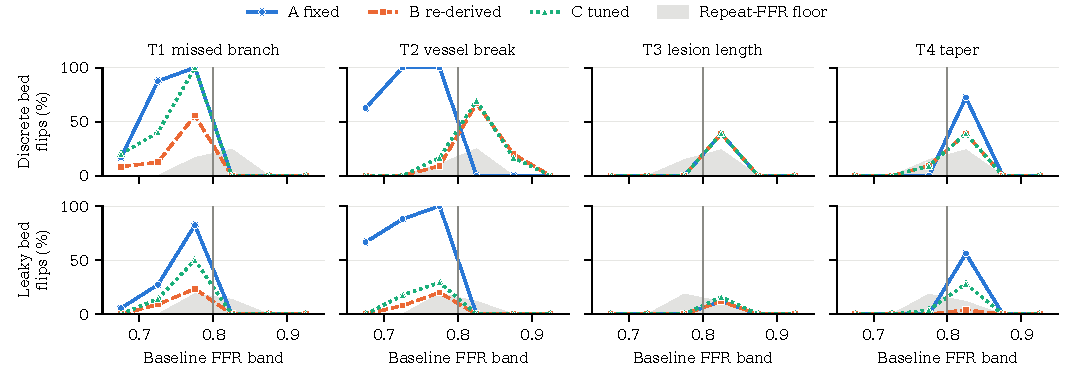
\includegraphics[width=\textwidth]{figures/fig2_flip_by_band.pdf}
\caption{Proportion of models whose classification at FFR 0.80 changed, by baseline FFR band (0.05 wide, plotted at
the band centre; bands with fewer than three models omitted), error type, protocol and bed structure. Shaded: flip
rate expected from repeat invasive FFR (standard deviation 0.018).}
\label{fig:band}
\end{figure*}

\subsection{Absorption Under Tuned Boundary Conditions}
Fitting one bed scaling to the clean territory flows (Protocol C) lowered the median perfusion residual of
topological-error models from 0.19 to 0.14 in the discrete bed and from 0.10 to 0.02 in the leaky bed. Compared with
Protocol A, tuning reversed 4 missed-branch flips and created none in each bed ($p = 0.25$). For vessel breaks it
reversed 32 flips and created none in the leaky bed ($p < 0.001$), and reversed 22 and created 10 in the discrete
bed ($p = 0.15$). Tuning therefore did not leave the flip rate at or above that of fixed boundary conditions; where
the change was resolved, it was a reduction.
Relative to re-derived boundary conditions (Protocol B), tuning changed at most two topological-error decisions per
cell ($p \geq 0.5$), while it lowered the median residual of missed-branch models from 0.36 to 0.16 (discrete) and
from 0.04 to 0.03 (leaky).

Tuning did not remove the error from the FFR (Fig.~\ref{fig:absorb}). Of the tuned topological-error models, 20 of
104 (19\%, 13--28\%) in the discrete bed and 14 of 171 (8\%, 5--13\%) in the leaky bed passed the perfusion check
while their FFR differed from the clean value by more than 0.05. In the discrete bed these were half of the 39
models that passed. Four and 12 of the passing models changed the decision. Under Protocol A the same proportions
were 12\% and 20\%; the ordering of A and C differed between the beds, so no difference between them is claimed. At
validation thresholds of 13\% and 16\%, the proportion under Protocol C rose to 28\% (20--37\%) and 38\% (30--48\%) in
the discrete bed and was 9\% (6--15\%) at both in the leaky bed.

Tuning also enlarged the taper error. In the leaky bed, 36 of 150 tuned taper models (24\%, 18--31\%) passed the
check while materially wrong, against 10 under Protocol A (Table~\ref{tab:results}).

\begin{figure}[!t]\centering
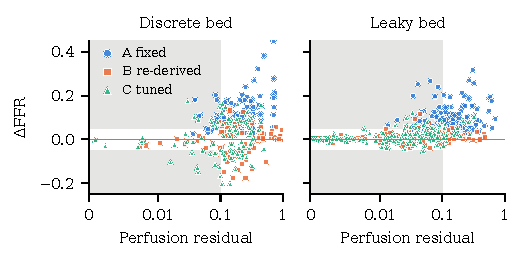
\includegraphics[width=\columnwidth]{figures/fig3_absorption.pdf}
\caption{Change in FFR against territory-perfusion residual for missed-branch and vessel-break models. Shaded:
models that pass the perfusion check (residual $< 0.10$) with $|\Delta\mathrm{FFR}| > 0.05$. Horizontal axis linear
below 0.01 and logarithmic above.}
\label{fig:absorb}
\end{figure}

\subsection{Side-Branch Loss Under Fixed and Tuned Resistance}
In the 44 (discrete) and 71 (leaky) instances in which Protocol C was defined, a missed side branch raised FFR by a
median of 0.095 and 0.047 with fixed boundary conditions. The shift exceeded 13\% of the clean FFR in 45\% and 11\%
of these instances. Tuning reduced the shift to a median of 0.077 and 0.015 (Wilcoxon signed-rank, $p < 0.001$ in
both beds; Fig.~\ref{fig:branch}). In the leaky bed the tuned shift was a median 42\% of the fixed shift, and 12 of
71 instances remained above 0.05. In the discrete bed it was 84\%, and 33 of 44 remained above 0.05.

\begin{figure}[!t]\centering
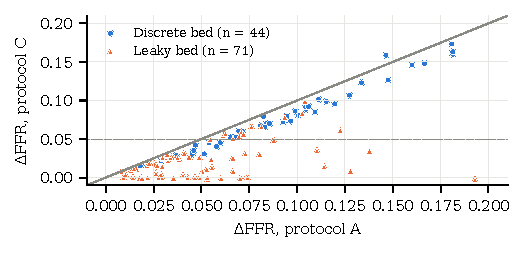
\includegraphics[width=\columnwidth]{figures/fig4_branch_loss.pdf}
\caption{Change in FFR caused by a missed side branch under fixed boundary conditions (Protocol A) and after tuning
to territory flows (Protocol C), paired by instance. Solid line: identity. Dashed line: $\Delta$FFR $= 0.05$.}
\label{fig:branch}
\end{figure}

\subsection{Three-Dimensional Case Study}
With the clean tree's resistances at the outlets, removal of the side branch raised the 3D FFR at the measurement
point from 0.870 to 0.944 ($\Delta$FFR $= +0.074$). With the clean territory flows prescribed at the outlets, the same
error changed FFR by $-0.0007$ (0.892 in both geometries). The
reduced-order twins gave $+0.081$ and $-0.0005$ for the same two conditions, and their baseline FFR was within 0.011
of the 3D values (Fig.~\ref{fig:case3d}).
\begin{figure}[!t]\centering
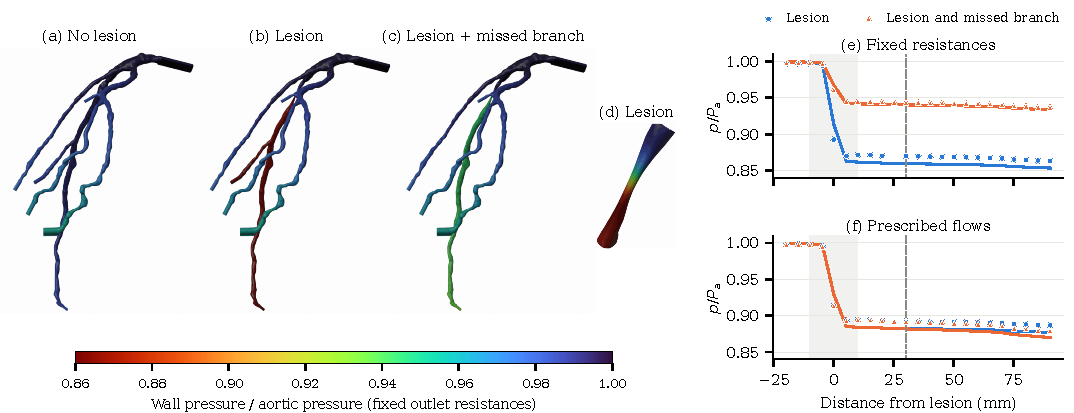
\includegraphics[width=\columnwidth]{figures/fig5_case3d.pdf}
\caption{Three-dimensional case study (proximal left anterior descending artery, 80\% DS): pressure along the host
vessel for the baseline and missed-branch lumens. Markers: 3D cross-section averages. Lines: reduced-order twins on
the meshed radius with the same outlet conditions. Shaded: lesion. Dashed: measurement point.}
\label{fig:case3d}
\end{figure} The meshed lumen was wider than the radius used by the reduced-order model
(median difference 0.14~mm; throat area-equivalent radius 0.276 against 0.231~mm), and on the requested radius the
reduced-order baseline was 0.761. Halving the cell size in the throat zone to 12.5~\textmu m changed the baseline
FFR by 0.0019 and 0.0021 in two zone placements, against the error effect of 0.074. A regenerated mesh at
25~\textmu m reproduced the baseline value.


% ---------------------------------------------------------------------------------------------------------------
\section{Discussion}
\subsection{Concealment at Calibration}
With fixed boundary conditions, a topological segmentation error changed the decision at 0.80 three to six times
as often as a calibre error of inter-observer magnitude, and the calibre errors produced flip rates of the order of repeat invasive measurement. The
decision risk of segmentation therefore lies mainly in the branching structure of the lumen, not in its calibre.

How much of a topological error reaches the decision depends on the boundary conditions. With the clean bed held
fixed, a missed branch or a vessel break flipped 18--43\% of decisions. Re-deriving the bed from the corrupted tree
reduced this to 5--18\%, and tuning one bed scaling to territory flows gave 8--20\%. The prediction that tuning leaves
the flip rate at or above that of fixed boundary conditions did not hold. Tuning moved the decision towards the
clean result.

Tuning did, however, separate the validation check from the error. Re-derived models carried the error in their
perfusion residual (median 0.36 for a missed branch in the discrete bed), so a perfusion check flagged them. Tuning
lowered that residual to 0.16 without changing more than two decisions per cell. In the discrete bed, half of the
tuned topological-error models that passed the check had an FFR error larger than 0.05. The check thus measured
agreement with the targets that were fitted, and the remaining error sat in the pressure distribution along the
vessel, which one global scaling cannot restore once a branch is absent. The same mechanism appeared in the
three-dimensional case: prescribing the clean territory flows reduced a missed-branch shift of 0.074 to $-0.0007$,
and the reduced-order twins reproduced both values.

Bed structure set the magnitude. In the leaky bed, the conductance of a deleted branch reappears as wall outflow at
its parent node, which damps the missed-branch error before any tuning. The discrete bed, which corresponds to the
outlet structure of a three-dimensional model, retained 84\% of the missed-branch shift after tuning. Claims in this
study are restricted to directions that held in both structures, and effect sizes are reported for each.

\subsection{Relation to Published Studies}
Published sensitivity analyses of computed FFR perturb lumen calibre with the branching structure fixed and report
continuous sensitivity \cite{sankaran2015tmi,sankaran2015cmame,fernandez2024,dalmaso2025}. Within that framework, our
calibre errors of inter-observer magnitude changed FFR by 0.006--0.037 on average and rarely changed the decision. Studies that compare
geometry with boundary conditions rank their influence on a continuous output \cite{sankaran2016,tanade2022,korte2023};
the present results add that the ranking depends on the error type and on the boundary-condition protocol, and that
the decision outcome separates them more clearly than the continuous one.

A side-branch effect of 13--15\% under fixed outlet resistance was reported from optical coherence tomography-based
models \cite{gamage2022}, and re-tuning the microvascular resistance absorbed a change in side-branch flow with little change in diagnostic
accuracy \cite{gosling2020}.
Both results were reproduced here within one cohort: the missed-branch shift exceeded 13\% of the clean FFR in 45\%
(discrete) and 11\% (leaky) of instances with fixed resistance, and tuning reduced it. The two earlier findings are
therefore consistent, and the difference between them follows from the boundary-condition protocol. A change of the
outlet model in a clinical computed-FFR cohort left the area under the curve unchanged while sensitivity changed
\cite{fossan2026}. The protocol effect observed here, up to a ninefold difference in flip rate on identical anatomy, is
consistent with that observation.

Overlap metrics barely register a missing branch, and vessel breaks occur in the output of current coronary
segmentation methods despite high overlap scores \cite{bransby2026}. The error types that carried the decision risk
in this study are the ones that overlap metrics do not measure.

\subsection{Implications for Model Validation}
Perfusion imaging is used to personalise and check coronary flow models \cite{menon2024}. In this study, passing a perfusion check
stricter than the repeatability of the measurement did not establish that the FFR was correct: 8--19\% of tuned
topological-error models passed with a material FFR error. The perfusion residual before tuning was informative,
because re-derived models carried a large residual when a branch was missing. Reporting the untuned residual beside
the tuned one, and reporting topological agreement of the segmentation (branch completeness and connectivity) beside
overlap, would expose errors that the tuned residual conceals.

\subsection{Limitations}
The stenoses were inserted into healthy vessels to obtain lesions near the threshold, so the lesion geometry is
idealised. The reduced-order model is steady, without autoregulation or heart-rate effects. The magnitudes of the
missed-branch and vessel-break errors are design choices; the calibre magnitudes come from inter-observer statistics
that are an upper bound on agreement. Protocol C used one global scaling, the least flexible tuning, and a
per-territory scaling was not evaluated. Protocol C was undefined for most right coronary instances with a
topological error, so the tuned-protocol results for these error types describe the left coronary tree. The
three-dimensional analysis covers one instance, and its meshed lumen was wider than the radius used by the
reduced-order model. No invasive FFR was available; the noise floor was modelled from published repeat measurements.

\section{Conclusion}
In 150 coronary trees with controlled stenoses and fixed boundary conditions, topological segmentation errors
changed the decision at FFR 0.80 three to six times as often as calibre errors of inter-observer magnitude, which were close to the repeatability of
invasive measurement. The boundary-condition protocol changed the flip rate of topological errors by up to a factor of nine. Tuning one bed scaling to territory flows reduced decision changes but removed the perfusion residual that
marked the error: 8--19\% of tuned models passed a perfusion check while their FFR was wrong by more than 0.05. A
three-dimensional case reproduced the masking of a missed side branch under prescribed flows.

\section*{Data and Code Availability}
ImageCAS-X is available under CC BY 4.0 (doi:10.5281/zenodo.21887809). Code and the frozen cohort: \textit{[DOI]}.

\section*{Acknowledgment}

\bibliographystyle{IEEEtran}
\bibliography{refs}

\end{document}
